\section{Objectives}

% The objective of this thesis is to find a reconciliation of the two goals, by finding an equivalence between two approaches with different goals, in the case of streaming web applications.

In section \ref{chapter3:software-design}, we show that the best organization to improve maintainability of an application is in a certain modularity.
This maintainability is further supported by a functional approach.
Indeed, higher-order functions play an important role in good modularity to improve readability and maintainability.
However, functional programming, and particularly higher-order functions, require the use of a global memory store.

In section \ref{chapter4:software-efficiency}, we show that to attain scalability, an application needs to be organized so as not to have a global memory store.
Still, many works try to provide this global memory store interface to developers, because it is the best way to support the modularity advocated in section \ref{chapter3:software-design}.
This incompatibility between these two organization, and their goals is responsible for the shifts operated during the life of an application.
Huge developing effort are made to translate manually from one organization into the other, when the most pressing need shift from maintainability to performance, or vice versa.

In section \ref{chapter4:reconciliations}, we show different tentatives to reconciles the two organizations.
Most are satisfactory for specific domains, such as the high-performance computing, where it is accepted to spend long time developing an application to use thousands of accelerators to compute heavy calculation, because the expected speedup is profitable, compared to develop an application for all these thousands accelerators.
However, none is satisfactory in the case of web applications.
Indeed, they all are too specific, and require too much from the developer to be accepted at a large scale.

% \comment{Here a table summarizing the different approaches, and the sweet spot.}

\begin{table}
\begin{tabular}{l|l|l|l}
             & Maintainability         & Performance           & Both\\\hline
General      & Functional Programming  & Message-passing       & Loop parallelization\\
Web          & Javascript              & Pipeline architecture & ø
\end{tabular}
\caption{Summary of the state of the art}
\label{tab:chapter3:objectives:summary}
\end{table}

Our objectives is to find an equivalence between these two organization, to be able to compile one into the other, specifically for the case of web applications.
To do so, we focus on the Javascript programming language, and specifically, the node.js interpreter.
We intend to split a node.js application into a parallel pipeline of stages.
Our contribution is organized in two chapters, as illustrated in figure \ref{fig:chapter3:objectives:roadmap}.
In the fourth chapter of this thesis, we present the extraction of a pipeline of stages from a Javascript application.
We show that such pipeline of operations is exposed by Promises, and we propose a simpler alternative to Promises : Dues.
However, these stages are not yet executed in parallel, and still require a global memory.
In the fifth chapter, we present the isolation of the stages of the pipeline into isolated containers called Fluxions. 

\begin{figure}[h!]
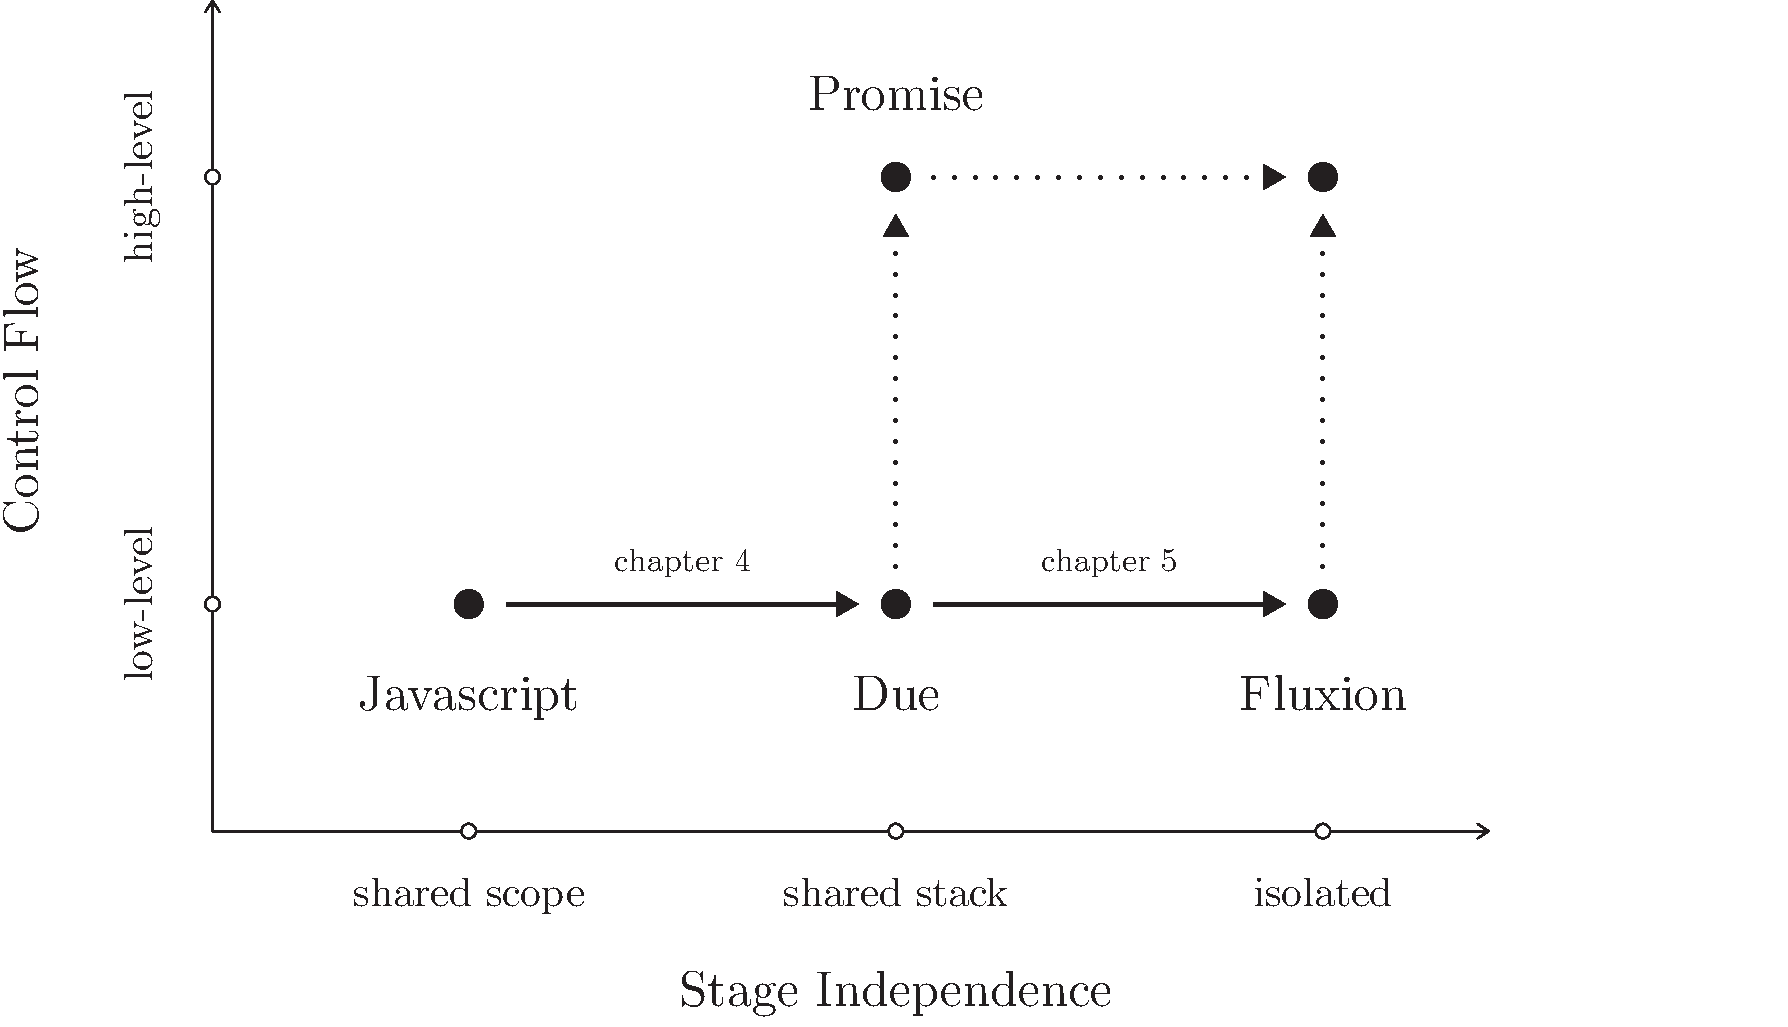
\includegraphics[width=1\textwidth]{../ressources/roadmap.pdf}
\caption{Roadmap for this work}
\label{fig:chapter3:objectives:roadmap}
\end{figure}

\endinput

We show that there is no languages that features higher-order functions to improve modularity, a common memory store easy to develop with, but at the same time provides scalable concurrency.

We aim at filling this gap, and for a concrete example, focus our work on the Javascript programing language.
Indeed, Javascript features higher-order functions, is highly-used in concurrent context, but lacks scalable concurrency.

Our work is divided into two contributions: Due and Fluxions.

-> Schema roadmap.